\section{FRONTEND}\label{ch:frontend}

Das Frontend wurde mithilfe der Frameworks Angular und Bootstrap entwickelt.
Mittels Angular wird eine Weboberfläche komponentenbasiert zur Verfügung gestellt.
Für die serverseitige Anwendung benötigt Angular zudem Node.js, eine JavaScript-Laufzeitumgebung.
Bootstrap bietet Vorlagen zur Gestaltung von Webseiten.

\subsection{Architektur}
Eine Komponente besteht aus einem Template (HTML-Datei) und einem Style (CSS-Datei). Diese werden als Metadaten im Dekorator der Komponente festgelegt und stellen die Ansicht dar.
Mithilfe der Datenbindung kann das Template mit der Komponente Daten austauschen und gegebenenfalls Events ausführen. In den Modulen werden Komponenten, Module, Services usw. gruppiert und verwaltet. In Angular werden zwei Modularten unterschieden. Jedes Angular Projekt besitzt ein Root-Modul, das \texttt{app.module.ts} heißt. Diese ist dazu da, um die gesamte Webanwendung zu verwalten und diese wird beim Start der Anwendung als erstes geladen und initialisiert. Im Root-Modul müssen alle erstellten Komponenten angegeben werden, damit diese in der Webanwendung angezeigt und geladen werden können. Als externes Modul wurde das \textbf{QuillModul} und \textbf{Angular Material} verwendet.

\begin{figure}[thpb]
      \centering
      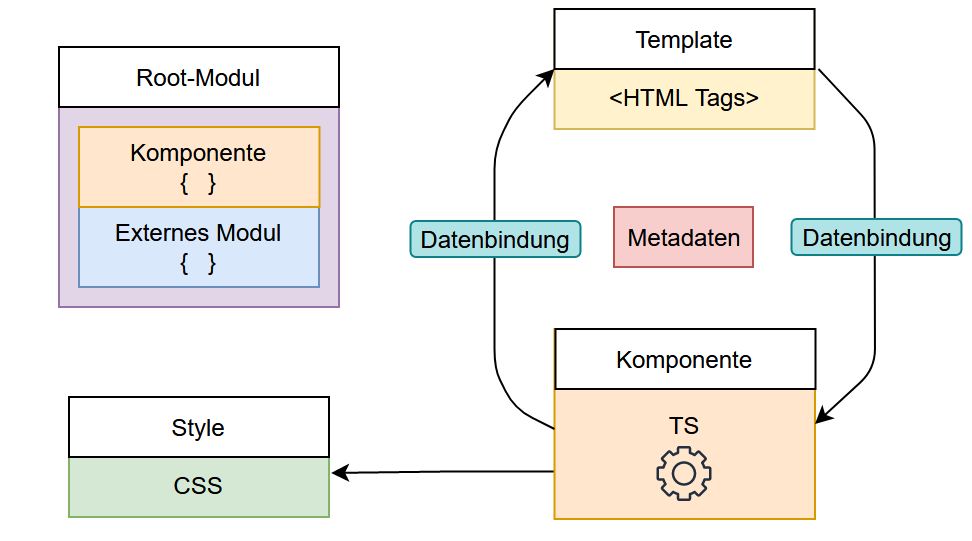
\includegraphics[scale=0.55]{abbildungen/angular_architektur.png}
      \caption{Angular Architektur des Projektes}
      \label{fig:frontend}
 \end{figure}

\subsection{Entwickelte Komponenten}
\begin{itemize}
\item \textbf{Artikel}: Holt sich einen Artikel über die \textbf{GET /article/\{id\}} Route und zeigt ihn in einer benutzerfreundlichen Ansicht an. Dabei wird ein Knopf zur Verfügung gestellt, über welchen dieser Artikel bearbeitet werden kann.
\item \textbf{Editor}: Wird der Editierknopf der Artikelkomponente gedrückt, beginnt eine weiterleitung über das Angular-Routing-Module zu dem Editor. Hier wurde der \textbf{Quill Rich Text Editor} eingebunden. 
Dieser bietet von Haus aus eine Reihe von Funktionalitäten über eine globale Config an.
Innerhalb dieses Editors wird der alte Artikeltext inklusive vollem CSS-Styling angezeigt. 
Ebenso lässt sich der Titel des Artikels über ein \textbf{Contenteditible-Event} anpassen. 
Des Weiteren wird unterhalb des Editors eine \textbf{Tag-Box} bereitgestellt, über die der User Tags hinzufügen und entfernen kann. Ist der User nun zufrieden mit seinen Anpassungen, kann er auf einen speichern Knopf drücken und die Änderungen über die \textbf{POST /articles/update} Route speichern oder seine Änderungen über einen abbrechen Knopf verwerfen. 
Diese Tag-Box wurden mittels Angular Material Chips umgesetzt.
\item \textbf{Header}: Die Header-Komponente beinhaltet einerseits die drei wichtigsten Weiterleitungen eines Studenten: Das \textbf{Moodle-Portal}, das \textbf{Primuss-Portal} und die \textbf{Webmail-Oberfläche}. Darüberhinaus wird ein Suchfeld angeboten, über das der Nutzer nach Artikeln oder Tags suchen kann.
\item \textbf{Sidebar}: Die Sidebar-Komponente gibt eine Übersicht über Kategorien, Unterkategorien und Artikeln. Durch Klick auf die dort angezeigten Artikel wird der User entsprechend auf diesen Artikel weitergeleitet. \\
$\rightarrow$ Mobile Ansicht für Header und Sidebar wurde mithilfe der Vorlagen von \textbf{Angular Material} entwickelt. Diesbezüglich wurden die HTML-Tags \texttt{<mat-toolbar>} und \texttt{<mat-sidenav>} genutzt.
\item \textbf{Footer}: Die Footer-Komponente zeigt einige Basisinformationen, wie die Datenschutzvereinbarung an. 
\item \textbf{Scroll-to-Top}: Diese Komponente stellt einen Knopf zur Verfügung, welchen den User direkt zum Seitenanfang befördert ohne selbst scrollen zu müssen. 
\end{itemize}

\subsection{Routing}
Das Routing in Angular ist dafür zuständig, dass Benutzer sich durch verschiedene Ansichten navigieren zu können. Dazu führt der Benutzer eine Aktion aus, wie zum Beispiel das Aufrufen eines Links, der zu einer neuen Seite navigiert oder die Eingabe einer URL. Im Routing können URL-Links fest definiert werden. Der Router weiß somit, welche Seite angefordert ist und ruft diese entsprechend auf.


